\documentclass{article}
\usepackage[utf8]{inputenc}
\usepackage{amsmath}
\usepackage{graphicx}
\usepackage{url}
\usepackage{tikz}
\usetikzlibrary{arrows.meta, positioning}
\usepackage{float}   % enables [H] figure placement
\usepackage{placeins} % enables \FloatBarrier
\title{Adaptive Learning System for CS Education\\("Google Maps for Learning")\\\large Research Report}
\author{Faiz Mustansar}
\date{January 5 -- April 2, 2026}

\begin{document}
\maketitle

% ============================
% BRIEF SUMMARY
% ============================

\section*{Brief Summary}
This project investigates the design and implementation of an adaptive learning
system for computer science (CS) education. The system estimates a learner’s
current knowledge state using Bayesian Knowledge Tracing, represents CS topics
as a prerequisite graph, generates a personalized learning route toward a target
goal, and dynamically updates that route as new evidence of learning is observed.
The research component draws on peer-reviewed literature in adaptive learning,
intelligent tutoring systems (ITS), student modeling, and knowledge tracing to
motivate and justify implementation decisions related to knowledge representation,
assessment design, routing logic, and evaluation. The project has produced a
fully functional MVP: a dockerized web application implementing the complete
adaptive learning loop, validated through unit and integration tests and
end-to-end walkthroughs of the learner flow.

\tableofcontents
\newpage

% ============================
% SECTION 1: BACKGROUND
% ============================

\section{Background}

% ---------- 1.1 ----------
\subsection{Adaptive Learning and Intelligent Tutoring Systems}

Adaptive learning systems aim to personalize instruction by adapting content
selection, sequencing, feedback, and pacing to individual learners. A central
idea across the literature is that adaptation is driven by a model of the learner,
which is updated using evidence from learner interactions and used to decide what
the learner should do next \cite{brusilovsky2001,woolf2009}. Unlike static curricula,
adaptive systems continuously incorporate new evidence (e.g., correctness,
attempt history, time-on-task) to provide recommendations that better reflect the
learner’s evolving knowledge state \cite{brusilovsky2001}.

A major research lineage formalizing adaptive learning is Intelligent Tutoring
Systems (ITS). ITS research typically decomposes instructional systems into four
core components: (i) a \textit{domain model} representing the target knowledge or
skills, (ii) a \textit{student model} representing what the learner currently
knows, (iii) a \textit{pedagogical model} specifying instructional decisions such
as feedback or task selection, and (iv) an \textit{interface model} that mediates
interaction with the learner \cite{woolf2009,vanlehn2006}. This decomposition is
particularly useful for implementation-focused projects, as it clarifies which
parts of the system estimate learning and which parts act on those estimates.

VanLehn further distinguishes between two adaptation loops within tutoring
systems: an \textit{outer loop}, which selects the next task or learning activity,
and an \textit{inner loop}, which provides step-level guidance during problem
solving \cite{vanlehn2006}. For adaptive systems that emphasize learning path
planning, such as the ``Google Maps for learning'' approach, the outer loop plays
a central role by determining sequencing and rerouting decisions. Prior work
suggests that robust outer-loop adaptation can yield meaningful benefits even
when inner-loop guidance is relatively simple, making it a practical focus for
term-scale prototypes \cite{vanlehn2006,woolf2009}.

Adaptive learning systems rely heavily on student modeling techniques to infer
latent knowledge states from observable behavior. Knowledge Tracing models, which
treat mastery as an unobserved variable inferred from learner responses, have been
widely used to support mastery learning and adaptive sequencing decisions
\cite{corbett1995}. More recent work extends these ideas to large-scale and
data-rich environments, demonstrating that continuous learner modeling can
support both prediction and personalization \cite{piech2015dkt}. These results
motivate the integration of explicit student models into adaptive CS learning
systems.

From an implementation perspective, adaptive systems must balance theoretical
expressiveness with practical constraints such as data quality, interpretability,
and robustness. Large-scale tutoring platforms highlight the importance of
transparent decision policies and defensible inference mechanisms, particularly
in educational contexts where instructors and learners must trust system behavior
\cite{feng2014assistments}. These considerations align with the goals of an
implementation-focused capstone project that prioritizes interpretable models,
explicit knowledge structures, and verifiable adaptation logic.

% ---------- 1.2 ----------
\subsection{Student Modeling and Knowledge Tracing}
\label{sec:background-bkt}

Adaptive learning systems require a representation of what a learner knows in order to
make defensible sequencing and feedback decisions. This representation is commonly called a
\textit{student model}: a computational estimate of the learner’s knowledge state that is updated
from observable interaction evidence (e.g., responses to questions, attempts on exercises, or
programming submissions). A key challenge is that knowledge is \textit{latent} (unobserved);
systems therefore infer mastery probabilistically from performance traces rather than directly
measuring understanding \cite{corbett1995}. In knowledge tracing, the objective is typically to
estimate a learner’s evolving mastery over a set of skills/knowledge components (KCs) and use
these estimates to guide instruction and sequencing \cite{corbett1995}.

\paragraph{Bayesian Knowledge Tracing (BKT).}
Bayesian Knowledge Tracing (BKT) is a widely used method for modeling student knowledge in
intelligent tutoring and adaptive learning systems. In its basic form, BKT treats each
Knowledge Component (KC) as a hidden (unobserved) state that represents whether a student
has mastered a specific skill or not. At any point in time, the system does not know this
state directly and must estimate it based on the student’s responses \cite{corbett1995}.

BKT is commonly modeled as a two-state process where a student moves from
\textit{not mastered} to \textit{mastered}. After each attempt at a question or exercise,
the system updates its belief $P(L_t)$, which represents the probability that the student
has mastered the skill at time $t$. This approach is especially suitable for
implementation-focused systems because it is simple, interpretable, and supports clear
decision rules, such as advancing the student when mastery is high or providing extra
practice when mastery remains low \cite{corbett1995}.

In the standard BKT model, each skill is described using four probabilities:
\begin{itemize}
    \item $P(L_0)$: the initial probability that the student already knows the skill
    \item $P(T)$: the probability that the student learns the skill after an attempt
    \item $P(G)$: the probability that the student answers correctly by guessing
    \item $P(S)$: the probability that the student answers incorrectly despite knowing the skill
\end{itemize}

When a student responds to an item at time $t$, where $Correct_t \in \{0,1\}$ indicates
whether the response was correct, BKT first updates the probability of mastery using
Bayes’ rule:
\[
P(L_t \mid Correct_t) =
\begin{cases}
\frac{P(L_{t-1})(1-P(S))}{P(L_{t-1})(1-P(S)) + (1-P(L_{t-1}))P(G)} & \text{if } Correct_t = 1 \\
\frac{P(L_{t-1})P(S)}{P(L_{t-1})P(S) + (1-P(L_{t-1}))(1-P(G))} & \text{if } Correct_t = 0
\end{cases}
\]

After this update, the model accounts for the possibility that the student learned the
skill as a result of the attempt:
\[
P(L_t) = P(L_t \mid Correct_t) + \bigl(1 - P(L_t \mid Correct_t)\bigr)P(T)
\]

In simple terms, this process uses each student response to update how confident the system
is that the student understands the skill, while accounting for guessing, mistakes, and
learning over time \cite{corbett1995}.

\paragraph{BKT in CS and Programming Contexts.}
BKT was originally studied in tutoring contexts where learners practiced procedural skills over time,
including programming-oriented tutoring environments \cite{corbett1995}. In CS education, BKT is
particularly relevant because systems can instrument repeated practice opportunities and map them to
KCs (e.g., conditionals, loops, indexing, recursion). Evidence may come from structured questions
or from programming exercises (test-case correctness, compilation success, repeated attempts). Modern
programming learning platforms also produce richer traces than binary correctness, motivating extensions
that incorporate additional signals or alternative models when feasible \cite{piech2015dkt}. For a
capstone-scale implementation, BKT remains a strong baseline because it provides a clear, testable bridge
between observed performance and actionable sequencing logic \cite{corbett1995}.

\paragraph{Implementation Guidance (Prototype-Oriented).}
For an implementation-focused prototype, BKT can be implemented reliably by specifying a clean data schema
and an explicit KC mapping:
\begin{itemize}
    \item \textbf{Define KCs:} Decide the set of skills (KCs) the system will track (e.g., 10--30 KCs for an
    intro CS unit). Each KC gets its own BKT state and parameters \cite{corbett1995}.
    \item \textbf{Map items to KCs:} Each quiz item or programming exercise should be tagged with one (or a small
    set of) KCs. The simplest approach is an expert-defined mapping for the initial prototype.
    \item \textbf{Collect evidence:} Store per-attempt logs: (learner\_id, item\_id, kc\_id, timestamp, correctness,
    optional features such as attempts/time/compilation status).
    \item \textbf{Initialize parameters:} Start with plausible priors (e.g., moderate guess/slip; conservative learning
    rate) and refine with small-scale fitting if data permits. If fitting is not feasible within the term, parameters
    should be justified via literature and validated through sanity checks (Section~\ref{sec:evaluation-plan}) \cite{vandesande2013}.
    \item \textbf{Decision thresholds:} Implement a transparent policy such as:
    advance if $P(L_t) \ge \tau_{mastery}$, remediate if $P(L_t) \le \tau_{low}$ after $k$ opportunities.
\end{itemize}

Figure~\ref{fig:adaptive-loop} illustrates the closed-loop logic expected in an adaptive system: evidence updates
a student model, which drives a decision policy for next actions. Figure~\ref{fig:bkt-latent} emphasizes BKT’s key
assumption: mastery is latent, so responses are treated as noisy observations (guess/slip) \cite{corbett1995}.

% ----- Diagram: Adaptive loop -----
\begin{figure}[h]
\centering
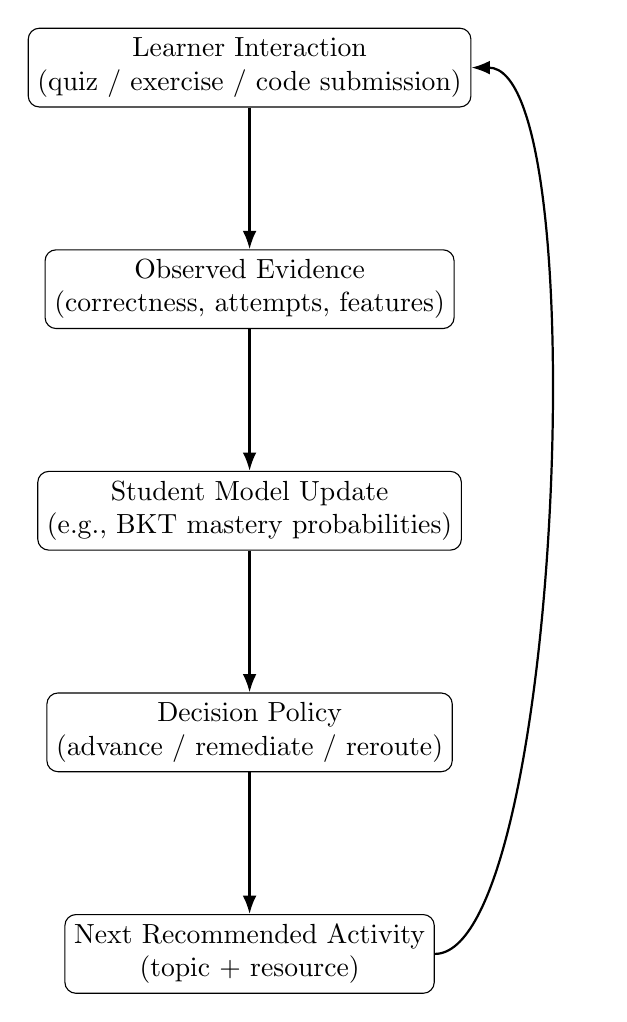
\begin{tikzpicture}[
  node distance=18mm,
  box/.style={draw, rounded corners, align=center, minimum width=4.2cm, minimum height=1cm},
  arrow/.style={-Latex, thick}
]
\node[box] (student) {Learner Interaction\\(quiz / exercise / code submission)};
\node[box, below=of student] (evidence) {Observed Evidence\\(correctness, attempts, features)};
\node[box, below=of evidence] (model) {Student Model Update\\(e.g., BKT mastery probabilities)};
\node[box, below=of model] (policy) {Decision Policy\\(advance / remediate / reroute)};
\node[box, below=of policy] (next) {Next Recommended Activity\\(topic + resource)};

\draw[arrow] (student) -- (evidence);
\draw[arrow] (evidence) -- (model);
\draw[arrow] (model) -- (policy);
\draw[arrow] (policy) -- (next);
\draw[arrow] (next.east) .. controls +(1.6,0) and +(1.6,0) .. (student.east);
\end{tikzpicture}
\caption{Closed-loop adaptation: interaction evidence updates the student model, which drives next-step decisions.}
\label{fig:adaptive-loop}
\end{figure}

% ----- Diagram: Latent mastery and observation in BKT -----
\begin{figure}[h]
\centering
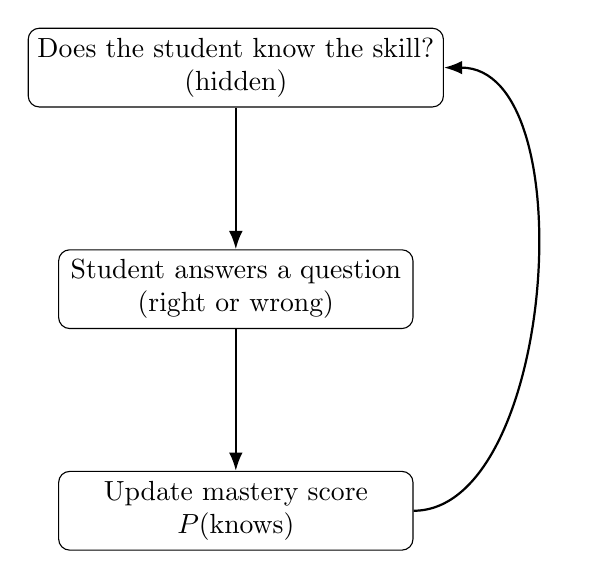
\begin{tikzpicture}[
  node distance=18mm,
  box/.style={draw, rounded corners, align=center, minimum width=4.5cm, minimum height=1cm},
  arrow/.style={-Latex, thick}
]
\node[box] (know) {Does the student know the skill?\\(hidden)};
\node[box, below=of know] (ans) {Student answers a question\\(right or wrong)};
\node[box, below=of ans] (update) {Update mastery score\\$P(\text{knows})$};

\draw[arrow] (know) -- (ans);
\draw[arrow] (ans) -- (update);
\draw[arrow] (update.east) .. controls +(1.8,0) and +(1.8,0) .. (know.east);
\end{tikzpicture}
\caption{Simple view of BKT: the system cannot directly see knowledge, so it uses answers to update a mastery score over time.}
\label{fig:bkt-simple}
\end{figure}


\paragraph{Limitations and Practical Pitfalls.}
Despite its usefulness, BKT has several limitations that matter in practice. First, standard BKT assumes
binary mastery and typically binary observations per KC opportunity, which can be reductive for CS tasks
where partial understanding and multi-step reasoning are common. Second, parameters can be sensitive and
may yield unrealistic mastery curves if poorly chosen or fit; analytic work shows that the behavior of BKT
can collapse into limited functional forms, and different parameter sets may produce similar predictions,
raising identifiability concerns \cite{vandesande2013}. Third, the independence assumptions in classic BKT
(e.g., skills modeled separately, opportunities treated similarly) can be violated in CS domains where
skills interact (e.g., loops and arrays) and where item difficulty varies significantly.

A common direction in the literature is to relax some of these assumptions by individualizing parameters
across students or incorporating richer features. For example, individualized BKT variants introduce
student-specific parameters to better capture heterogeneity in prior knowledge or learning rates, improving
predictive performance compared to skill-only parameterization \cite{yudelson2013ibkt}. More expressive
approaches such as Deep Knowledge Tracing replace explicit BKT structure with sequence models that can capture
complex dependencies; however, these methods often trade interpretability for accuracy and require more data
and careful validation \cite{piech2015dkt}. For this project, BKT is a defensible baseline because it is
transparent and implementable, while still allowing incremental extensions if sufficient data and time become
available \cite{corbett1995,vandesande2013,yudelson2013ibkt}.


% ---------- 1.3 ----------
\subsection{CS Knowledge Structure and Prerequisite Representation}
\label{sec:background-prereqs}

Computer science (CS) domains are naturally structured around prerequisite
relationships: learners must understand simpler concepts before progressing to
more complex abstractions (e.g., variables before conditionals, conditionals
before loops, loops before recursion). This hierarchical dependency structure
makes CS education particularly well-suited to graph-based knowledge
representations and path-planning approaches \cite{koedinger2012,robins2003}.

From an adaptive learning perspective, the ability to explicitly encode
prerequisites enables systems to reason about \textit{where a learner is}, what
they are \textit{ready to learn next}, and how to \textit{reroute} instruction
when learning difficulties are detected. This aligns directly with the
``Google Maps for learning'' metaphor: the learner’s current mastery state
determines their location on a map, while prerequisite constraints define which
routes are legally traversable \cite{brusilovsky2001}.

\paragraph{Knowledge Components (KCs).}
A foundational design decision is how to decompose CS content into
\textit{knowledge components} (KCs). KCs are the smallest units of knowledge or
skill that can be meaningfully practiced and assessed independently
\cite{koedinger2012}. In introductory CS contexts, examples include:
\begin{itemize}
    \item Variables and assignment
    \item Boolean expressions
    \item Conditional branching
    \item Iteration (for/while loops)
    \item Functions and parameter passing
    \item Arrays or lists
    \item Recursion
\end{itemize}

Each KC serves as a node in the system’s domain model and is tracked independently
by the student model (e.g., one BKT instance per KC). The granularity of KCs
represents a trade-off: coarse KCs reduce modeling complexity but may obscure
specific misconceptions, while overly fine-grained KCs increase annotation and
parameterization burden \cite{koedinger2012,robins2003}. For a term-scale
prototype, an expert-defined KC set grounded in standard CS curricula provides a
defensible and implementable compromise.

\paragraph{Prerequisite Graph Representation.}
Once KCs are defined, prerequisite relationships can be encoded as a directed
graph $G = (V, E)$, where each node $v \in V$ corresponds to a KC and each directed
edge $(u \rightarrow v) \in E$ indicates that mastery of $u$ is required before
learning $v$. In many introductory CS domains, this graph can be approximated as
a directed acyclic graph (DAG), simplifying routing and validation logic
\cite{koedinger2012}.

Figure~\ref{fig:cs-prereq-graph} illustrates a simplified prerequisite graph for
introductory programming concepts. Such a structure allows the system to:
(i) determine which nodes are currently available given a learner’s mastery
state, (ii) identify unmet prerequisites for a target goal, and (iii) generate
valid learning routes that respect dependency constraints.

% ----- Diagram: CS prerequisite graph -----
\begin{figure}[h]
\centering
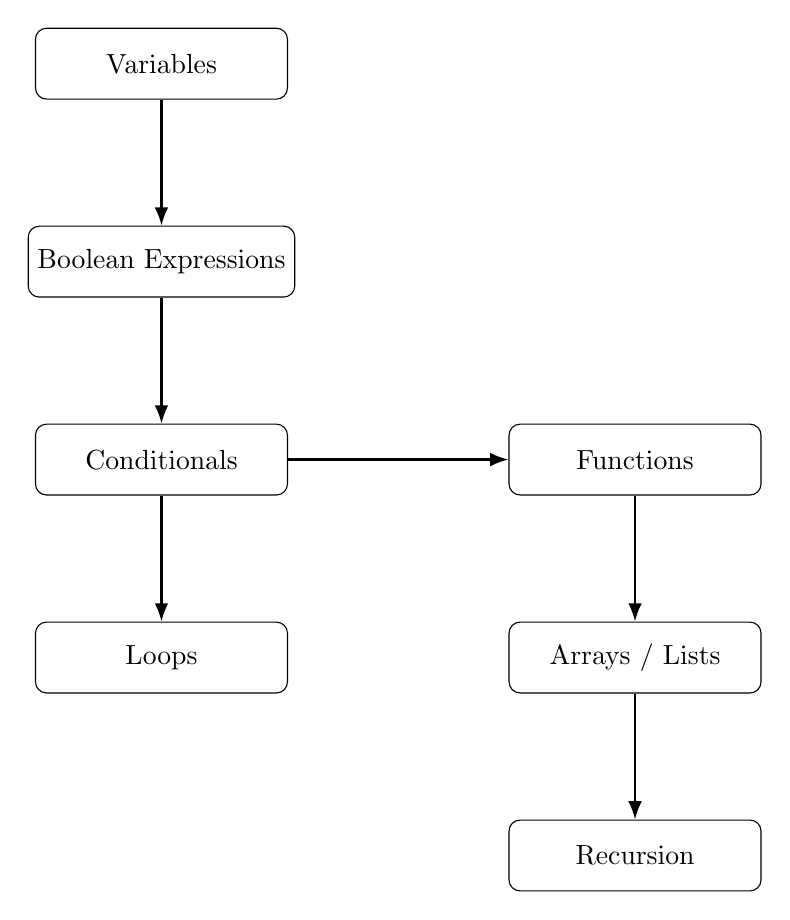
\begin{tikzpicture}[
  node distance=16mm,
  box/.style={draw, rounded corners, align=center, minimum width=3.2cm, minimum height=0.9cm},
  arrow/.style={-Latex, thick}
]

\node[box] (vars) {Variables};
\node[box, below=of vars] (bool) {Boolean Expressions};
\node[box, below=of bool] (cond) {Conditionals};
\node[box, below=of cond] (loops) {Loops};

\node[box, right=28mm of cond] (func) {Functions};
\node[box, below=of func] (arrays) {Arrays / Lists};
\node[box, below=of arrays] (rec) {Recursion};

\draw[arrow] (vars) -- (bool);
\draw[arrow] (bool) -- (cond);
\draw[arrow] (cond) -- (loops);

\draw[arrow] (cond) -- (func);
\draw[arrow] (func) -- (arrays);
\draw[arrow] (arrays) -- (rec);

\end{tikzpicture}
\caption{Example prerequisite graph for introductory CS concepts. Nodes represent
knowledge components; edges represent prerequisite relationships.}
\label{fig:cs-prereq-graph}
\end{figure}

\paragraph{Learning Path Planning as Graph Routing.}
Given a prerequisite graph and a learner’s estimated mastery state, learning path
generation can be formalized as a constrained routing problem. The system seeks a
path from the learner’s current location (set of mastered nodes) to a target goal
node, subject to prerequisite constraints. In its simplest form, this can be
implemented as rule-based prerequisite satisfaction: repeatedly select the
nearest unmet prerequisite until all prerequisites for the target are satisfied
\cite{brusilovsky2001}.

More advanced formulations treat routing as a graph search problem, where nodes
have associated costs derived from mastery probabilities, topic difficulty, or
estimated learning effort. Such formulations allow the system to compare multiple
valid routes and select one that optimizes a chosen objective (e.g., minimal
expected remediation) \cite{brusilovsky2001}. For a capstone-scale system, a
rule-based or breadth-first prerequisite expansion provides sufficient
adaptivity while remaining transparent and debuggable.

\paragraph{Integration with Student Modeling.}
Prerequisite graphs interact tightly with student models such as BKT. Mastery
estimates determine which nodes are considered ``complete,'' ``available,'' or
``blocked.'' When a learner repeatedly fails to demonstrate mastery on a KC, the
system can reroute by moving backward in the graph to reinforce prerequisites.
Conversely, when mastery probabilities exceed a threshold, the system may unlock
downstream nodes and advance the learning route. This explicit coupling between
graph structure and mastery inference operationalizes adaptive sequencing in a
way that is both explainable and implementable \cite{corbett1995,koedinger2012}.

\paragraph{Limitations and Design Risks.}
Despite their usefulness, prerequisite graphs impose simplifying assumptions.
First, real learning dependencies may not be strictly hierarchical; some CS
concepts are mutually reinforcing rather than linearly ordered. Second, expert-
defined graphs risk encoding instructor bias and may not reflect how learners
actually acquire skills \cite{koedinger2012}. Third, prerequisite satisfaction
alone does not capture differences in instructional effectiveness or learner
preferences.

To mitigate these limitations, this project treats the prerequisite graph as an
initial scaffold rather than a ground truth. The graph is intended to be small,
transparent, and revisable, allowing future extensions such as data-driven edge
validation or dynamic prerequisite relaxation. Within the scope of this project,
a carefully designed expert graph provides a practical foundation for adaptive
routing while keeping the system interpretable and robust.


\subsection{Course Chatbots and General-Purpose Generative AI (In Progress)}

In recent years, several universities and educational platforms have introduced
course-specific chatbots to support student learning. These systems are typically
designed to answer frequently asked questions, summarize course materials, or
provide clarifications about assignments and deadlines. In some cases, they are
trained on lecture slides, textbooks, or discussion forum content to offer
context-aware responses. While useful as instructional support tools, these
course chatbots generally do not model student knowledge or provide structured,
adaptive tutoring.

Unlike Intelligent Tutoring Systems, most university-deployed chatbots do not
maintain a persistent student model, track mastery over individual skills, or
adapt content sequencing based on learner performance. Their primary function is
information retrieval or explanation rather than instructional decision-making.
As a result, these systems offer limited guidance on what a student should learn
next or how their understanding evolves over time.

General-purpose generative AI systems such as ChatGPT, Claude, and Gemini further
extend conversational capabilities by providing natural language explanations,
code examples, and conceptual guidance across a wide range of topics. These tools
have demonstrated strong performance in explaining programming concepts and
assisting with debugging. However, they operate without explicit knowledge of a
learner’s prior understanding, progress, or misconceptions. Responses are
generated independently for each interaction, with no guaranteed consistency or
alignment to a structured curriculum.

From an educational modeling perspective, general-purpose language models lack
explicit representations of prerequisite relationships, mastery thresholds, and
learning objectives. While they may simulate tutoring behavior through dialogue,
they do not implement formal student modeling or adaptive sequencing policies.
This limits their ability to provide reliable learning paths or to justify
instructional decisions in a transparent way.

The proposed system differs from both course chatbots and general-purpose
generative AI by combining adaptive student modeling with an explicit knowledge
map of CS concepts. Rather than answering isolated questions, the system tracks
mastery at the level of individual knowledge components and uses this information
to generate and update personalized learning routes. Generative AI tools may be
used as supportive components (e.g., explanation or feedback generation), but the
core adaptivity logic is driven by interpretable models such as Bayesian Knowledge
Tracing and prerequisite-based routing.

This distinction positions the system closer to classical intelligent tutoring
systems while incorporating modern interaction paradigms. By separating
instructional decision-making from explanation generation, the system aims to
provide adaptive guidance that is both personalized and pedagogically grounded,
addressing limitations observed in existing chatbot-based educational tools.


% ============================
% SECTION 3: PROPOSED SYSTEM DESIGN
% ============================

% ============================
% SECTION 3: PROPOSED SYSTEM DESIGN
% ============================

\section{Proposed System Design (System Design Only)}
\label{sec:system-design}

\subsection{Design Goals and Scope}
This section specifies a term-scale, implementation-ready system design for an adaptive CS learning
platform. The design prioritizes (i) interpretability, (ii) explicit knowledge representation via a
prerequisite graph, and (iii) transparent decision-making for sequencing and rerouting. Adaptation is
driven by a student model (Bayesian Knowledge Tracing) operating over a set of instructor-defined
Knowledge Components (KCs), consistent with established ITS decompositions and outer-loop sequencing
logic \cite{woolf2009,vanlehn2006,corbett1995}.

\paragraph{Prototype scope (v1).}
The v1 system supports goal selection, diagnostic initialization, quiz/exercise attempts, mastery updates,
and prerequisite-respecting route generation. To reduce ambiguity in mastery updates and ensure clean
instrumentation, each activity item is mapped to exactly one KC in v1.

\paragraph{Out of scope (v1).}
Deep sequence models (e.g., DKT), automated KC discovery, multi-KC credit assignment, and sophisticated
step-level tutoring (inner-loop guidance) are deferred in favor of reliable outer-loop routing and
mastery tracking \cite{piech2015dkt,vanlehn2006}.

\FloatBarrier

% ----------------------------
% 3.1 System Overview Diagram
% ----------------------------
\subsection{System Architecture Overview}
Figure~\ref{fig:sys-overview} presents the system-level architecture. Learners interact with a map-based UI,
while instructors/admins define KCs, prerequisite edges, and an item bank. A backend API mediates all access,
persists events, and orchestrates routing and student-model updates.

\begin{figure}[H]
\centering
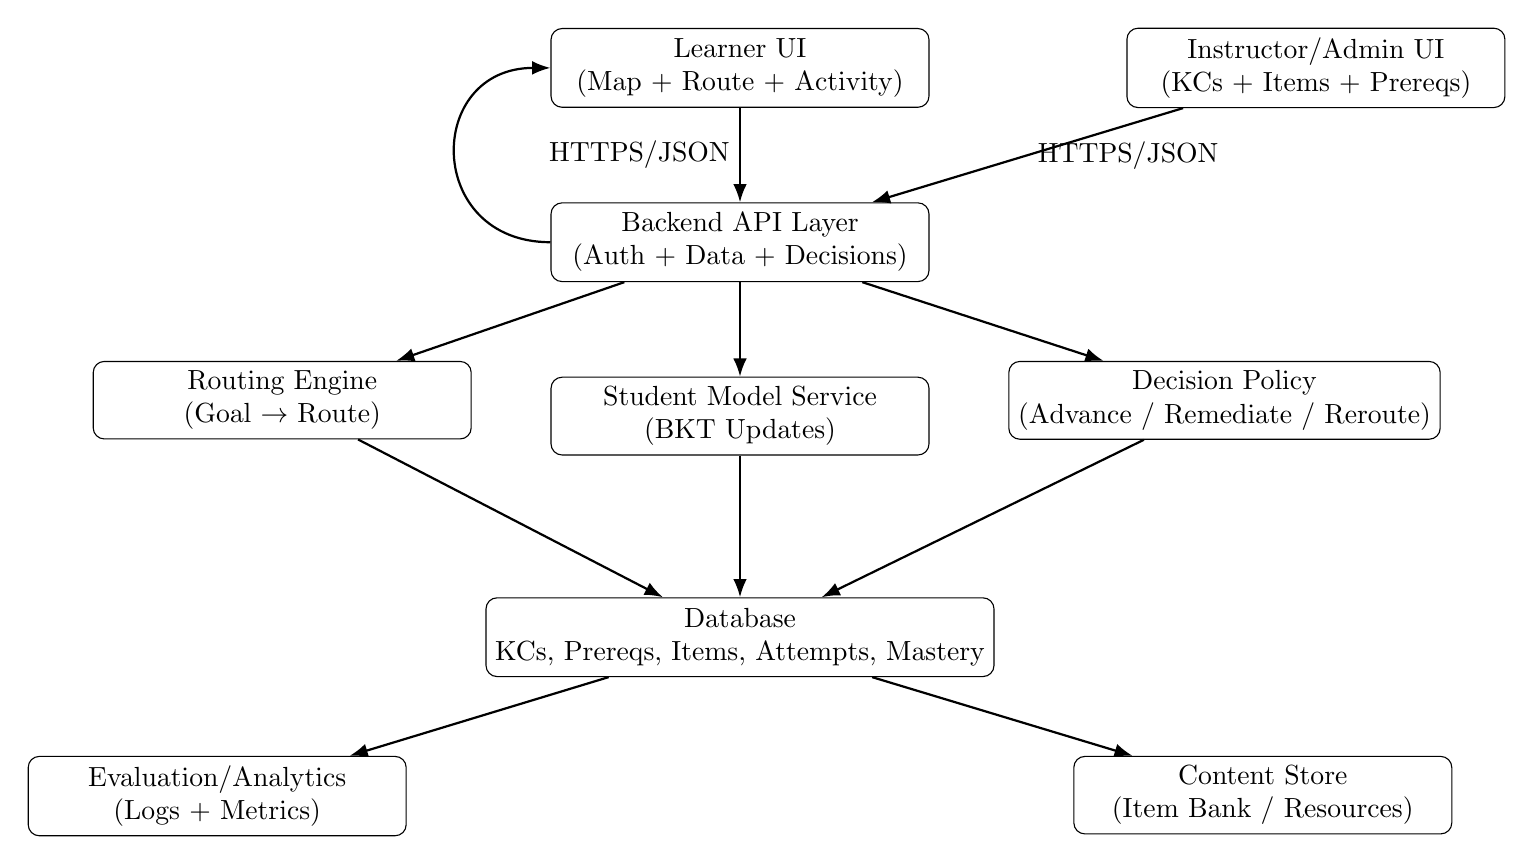
\begin{tikzpicture}[
  node distance=12mm,
  box/.style={draw, rounded corners, align=center, minimum width=4.8cm, minimum height=1.0cm},
  smallbox/.style={draw, rounded corners, align=center, minimum width=4.8cm, minimum height=0.85cm},
  arrow/.style={-Latex, thick}
]
\node[box] (ui) {Learner UI\\(Map + Route + Activity)};
\node[box, right=25mm of ui] (admin) {Instructor/Admin UI\\(KCs + Items + Prereqs)};

\node[box, below=of ui] (api) {Backend API Layer\\(Auth + Data + Decisions)};
\node[smallbox, below left=10mm and 10mm of api] (routing) {Routing Engine\\(Goal $\rightarrow$ Route)};
\node[smallbox, below=of api] (studentmodel) {Student Model Service\\(BKT Updates)};
\node[smallbox, below right=10mm and 10mm of api] (policy) {Decision Policy\\(Advance / Remediate / Reroute)};

\node[box, below=18mm of studentmodel] (db) {Database\\KCs, Prereqs, Items, Attempts, Mastery};

\node[smallbox, below left=10mm and 10mm of db] (eval) {Evaluation/Analytics\\(Logs + Metrics)};
\node[smallbox, below right=10mm and 10mm of db] (content) {Content Store\\(Item Bank / Resources)};

\draw[arrow] (ui) -- node[left]{HTTPS/JSON} (api);
\draw[arrow] (admin) -- node[right]{HTTPS/JSON} (api);

\draw[arrow] (api) -- (routing);
\draw[arrow] (api) -- (studentmodel);
\draw[arrow] (api) -- (policy);

\draw[arrow] (routing) -- (db);
\draw[arrow] (studentmodel) -- (db);
\draw[arrow] (policy) -- (db);

\draw[arrow] (db) -- (eval);
\draw[arrow] (db) -- (content);

\draw[arrow] (api.west) .. controls +(-1.6,0) and +(-1.6,0) .. (ui.west);
\end{tikzpicture}
\caption{System-level architecture for the adaptive learning platform.}
\label{fig:sys-overview}
\end{figure}

\paragraph{Key services.}
\begin{itemize}
    \item \textbf{Routing Engine:} constructs prerequisite-respecting learning routes from current mastery to a goal KC.
    \item \textbf{Student Model Service:} maintains per-learner mastery probabilities using BKT updates \cite{corbett1995}.
    \item \textbf{Decision Policy:} converts mastery signals into actions (advance, remediate, reroute) using transparent thresholds.
\end{itemize}

\FloatBarrier

% ---------------------------------
% 3.2 Learning Flow / State Machine
% ---------------------------------
\subsection{End-to-End Learning Flow}
Figure~\ref{fig:learning-flow} describes the outer-loop learning flow. The learner selects a goal KC, completes
a diagnostic to initialize mastery priors, follows the recommended route, and repeatedly updates mastery after
each attempt. The system reroutes when evidence indicates persistent low mastery.

\begin{figure}[H]
\centering
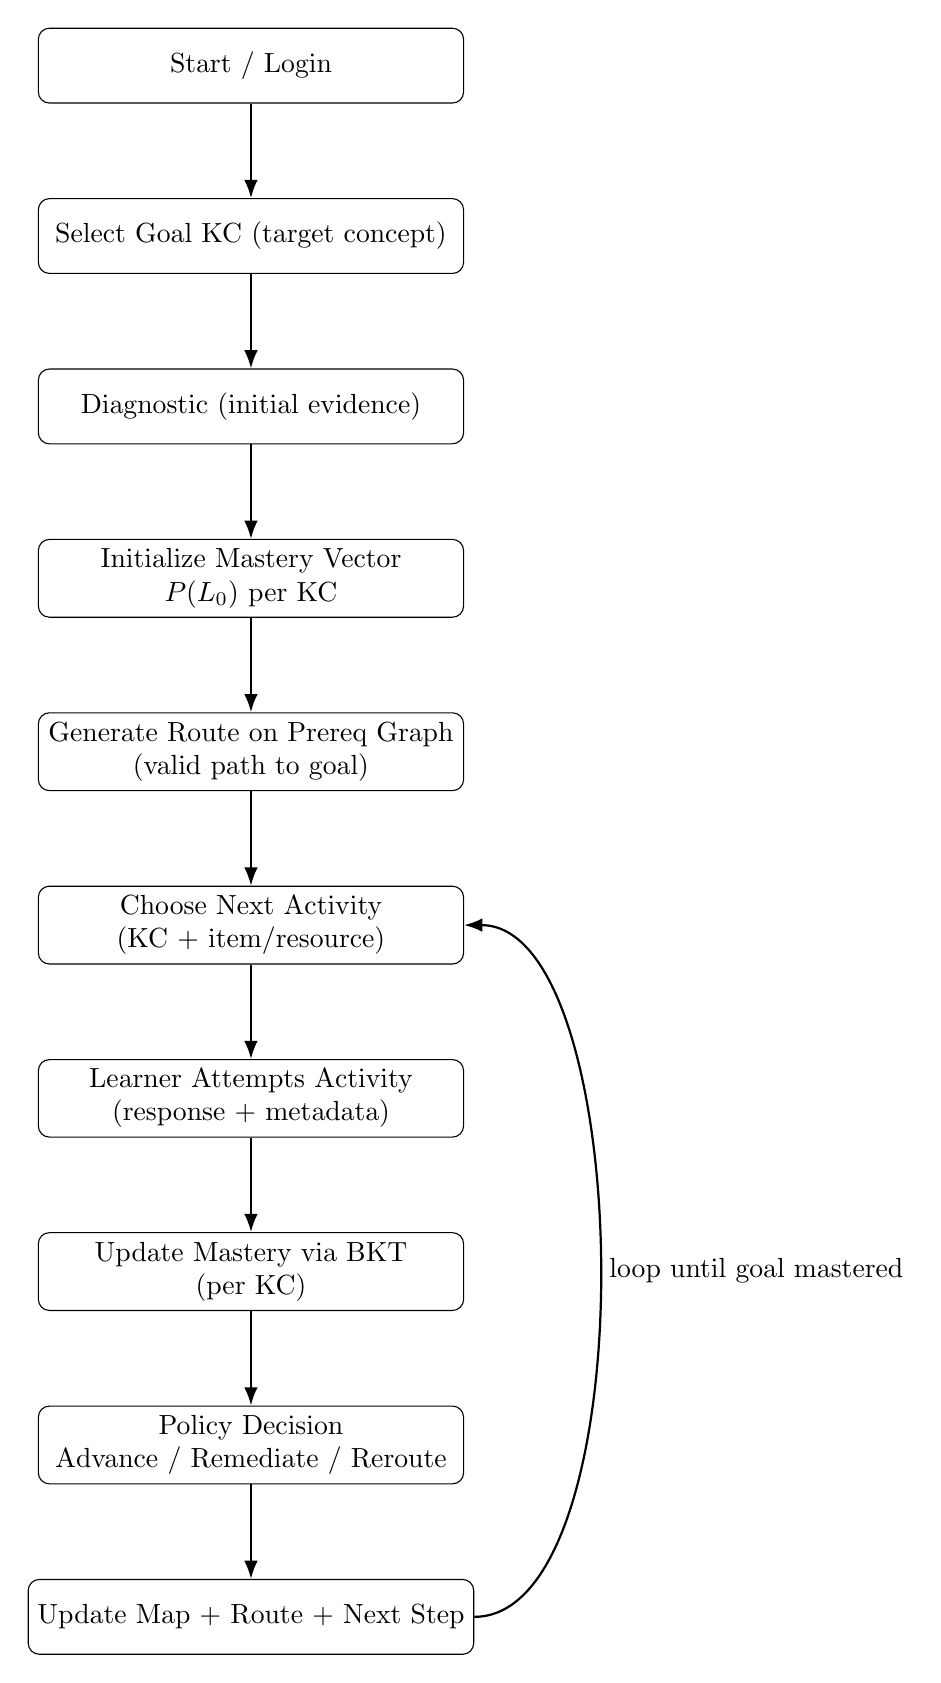
\begin{tikzpicture}[
  node distance=12mm,
  box/.style={draw, rounded corners, align=center, minimum width=5.4cm, minimum height=0.95cm},
  arrow/.style={-Latex, thick}
]
\node[box] (start) {Start / Login};
\node[box, below=of start] (selectgoal) {Select Goal KC (target concept)};
\node[box, below=of selectgoal] (diagnostic) {Diagnostic (initial evidence)};
\node[box, below=of diagnostic] (initmastery) {Initialize Mastery Vector\\$P(L_0)$ per KC};
\node[box, below=of initmastery] (route) {Generate Route on Prereq Graph\\(valid path to goal)};
\node[box, below=of route] (nextactivity) {Choose Next Activity\\(KC + item/resource)};
\node[box, below=of nextactivity] (attempt) {Learner Attempts Activity\\(response + metadata)};
\node[box, below=of attempt] (update) {Update Mastery via BKT\\(per KC)};
\node[box, below=of update] (decision) {Policy Decision\\Advance / Remediate / Reroute};
\node[box, below=of decision] (refresh) {Update Map + Route + Next Step};

\draw[arrow] (start) -- (selectgoal);
\draw[arrow] (selectgoal) -- (diagnostic);
\draw[arrow] (diagnostic) -- (initmastery);
\draw[arrow] (initmastery) -- (route);
\draw[arrow] (route) -- (nextactivity);
\draw[arrow] (nextactivity) -- (attempt);
\draw[arrow] (attempt) -- (update);
\draw[arrow] (update) -- (decision);
\draw[arrow] (decision) -- (refresh);
\draw[arrow] (refresh.east) .. controls +(2.2,0) and +(2.2,0) .. node[right]{loop until goal mastered} (nextactivity.east);

\end{tikzpicture}
\caption{End-to-end learning flow: diagnostic $\rightarrow$ route $\rightarrow$ practice $\rightarrow$ BKT update $\rightarrow$ decision $\rightarrow$ reroute.}
\label{fig:learning-flow}
\end{figure}

\paragraph{Diagnostic initialization.}
The diagnostic provides initial evidence to set $P(L_0)$ values per KC. In v1, the diagnostic can be implemented
as a small set of KC-tagged items; mastery priors are initialized using either fixed priors or diagnostic-derived
posteriors (same BKT update rule).

\FloatBarrier

% ----------------------------
% 3.3 Core Data Entities
% ----------------------------
\subsection{Core Data Model}
The platform uses a minimal relational schema that supports trace logging (attempts), mastery estimation, and
route computation. Figure~\ref{fig:data-entities} summarizes the core entities.

\begin{figure}[H]
\centering
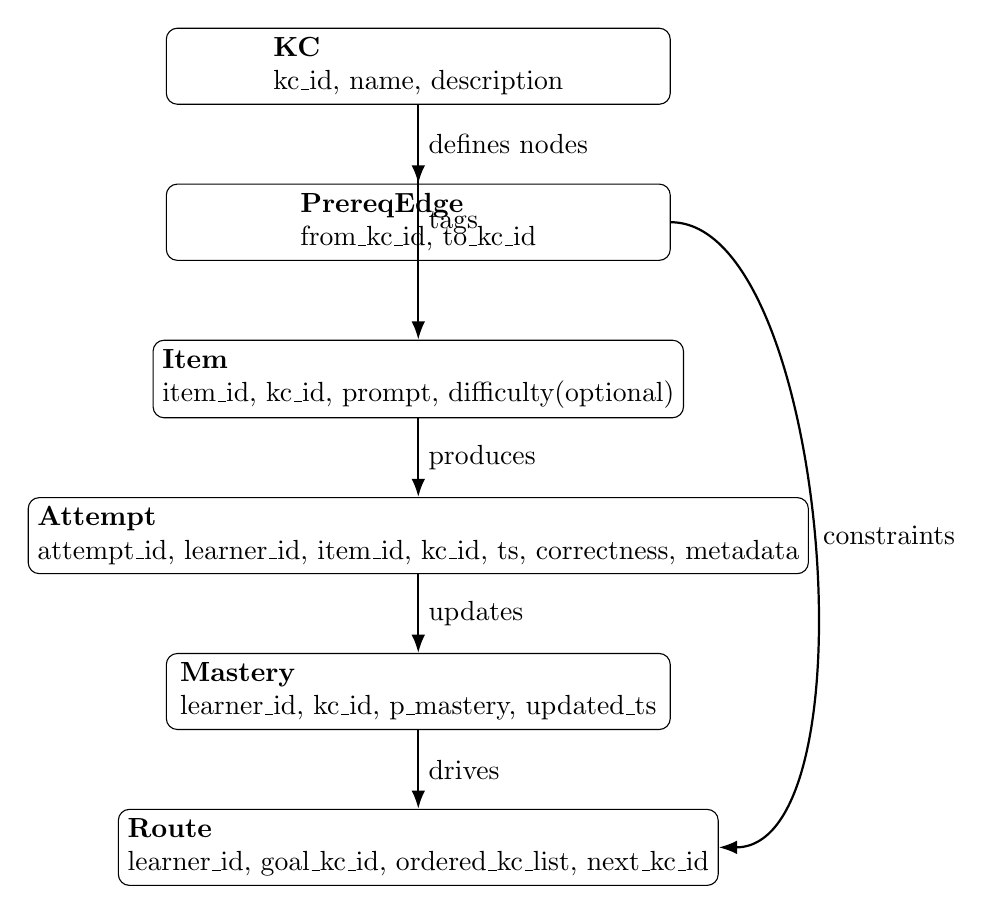
\begin{tikzpicture}[
  node distance=10mm,
  box/.style={draw, rounded corners, align=left, minimum width=6.4cm, minimum height=0.9cm},
  arrow/.style={-Latex, thick}
]
\node[box] (kc) {\textbf{KC}\\kc\_id, name, description};
\node[box, below=of kc] (edge) {\textbf{PrereqEdge}\\from\_kc\_id, to\_kc\_id};
\node[box, below=of edge] (item) {\textbf{Item}\\item\_id, kc\_id, prompt, difficulty(optional)};
\node[box, below=of item] (attempt) {\textbf{Attempt}\\attempt\_id, learner\_id, item\_id, kc\_id, ts, correctness, metadata};
\node[box, below=of attempt] (mastery) {\textbf{Mastery}\\learner\_id, kc\_id, p\_mastery, updated\_ts};
\node[box, below=of mastery] (route) {\textbf{Route}\\learner\_id, goal\_kc\_id, ordered\_kc\_list, next\_kc\_id};

\draw[arrow] (kc) -- node[right]{defines nodes} (edge);
\draw[arrow] (kc) -- node[right]{tags} (item);
\draw[arrow] (item) -- node[right]{produces} (attempt);
\draw[arrow] (attempt) -- node[right]{updates} (mastery);
\draw[arrow] (mastery) -- node[right]{drives} (route);
\draw[arrow] (edge.east) .. controls +(2.0,0) and +(2.0,0) .. node[right]{constraints} (route.east);

\end{tikzpicture}
\caption{Core data objects used by the system.}
\label{fig:data-entities}
\end{figure}

\paragraph{Item-to-KC mapping (v1 constraint).}
Each item is tagged to exactly one KC. This ensures that each attempt triggers a single BKT update and avoids
multi-skill credit assignment in the prototype.

\FloatBarrier

% ----------------------------
% 3.4 BKT Update Micro-Flow
% ----------------------------
\subsection{Student Model Service: BKT Update}
Mastery is modeled independently per KC using Bayesian Knowledge Tracing \cite{corbett1995}. Each attempt produces
a binary observation (correct/incorrect) and updates $P(L_t)$ for the attempted KC using Bayes' rule with guess and
slip, followed by the learning transition. Figure~\ref{fig:bkt-microflow} shows the update micro-flow.

\begin{figure}[H]
\centering
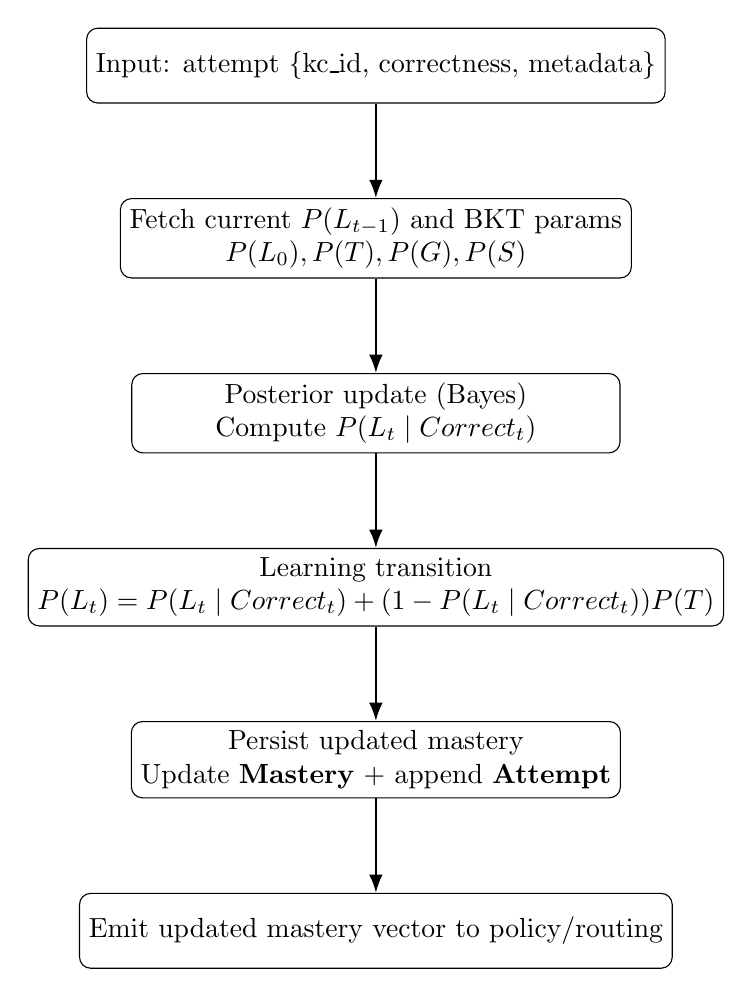
\begin{tikzpicture}[
  node distance=12mm,
  box/.style={draw, rounded corners, align=center, minimum width=6.2cm, minimum height=0.95cm},
  arrow/.style={-Latex, thick}
]
\node[box] (in) {Input: attempt \{kc\_id, correctness, metadata\}};
\node[box, below=of in] (fetch) {Fetch current $P(L_{t-1})$ and BKT params\\$P(L_0), P(T), P(G), P(S)$};
\node[box, below=of fetch] (bayes) {Posterior update (Bayes)\\Compute $P(L_t \mid Correct_t)$};
\node[box, below=of bayes] (learn) {Learning transition\\$P(L_t) = P(L_t \mid Correct_t) + (1 - P(L_t \mid Correct_t))P(T)$};
\node[box, below=of learn] (persist) {Persist updated mastery\\Update \textbf{Mastery} + append \textbf{Attempt}};
\node[box, below=of persist] (emit) {Emit updated mastery vector to policy/routing};

\draw[arrow] (in) -- (fetch);
\draw[arrow] (fetch) -- (bayes);
\draw[arrow] (bayes) -- (learn);
\draw[arrow] (learn) -- (persist);
\draw[arrow] (persist) -- (emit);

\end{tikzpicture}
\caption{Micro-flow for updating mastery probabilities using BKT after each learner attempt.}
\label{fig:bkt-microflow}
\end{figure}

\paragraph{BKT parameterization.}
In v1, BKT parameters may be set globally (shared across KCs) or per-KC using instructor-configured defaults.
Parameter fitting is optional; if fitting is not feasible within the term, parameters are justified via literature
and validated via sanity checks on mastery trajectories \cite{corbett1995,vandesande2013}.

\FloatBarrier

% ----------------------------
% 3.5 Routing + Rerouting Logic
% ----------------------------
\subsection{Routing Engine and Rerouting Policy}
Routing generates an ordered list of KCs leading from the learner's current mastery state to a goal KC while
respecting prerequisite constraints. The system treats a KC as ``mastered'' when $P(L) \ge \tau_{mastery}$.
Figure~\ref{fig:routing-logic} summarizes the routing logic.

\begin{figure}[H]
\centering
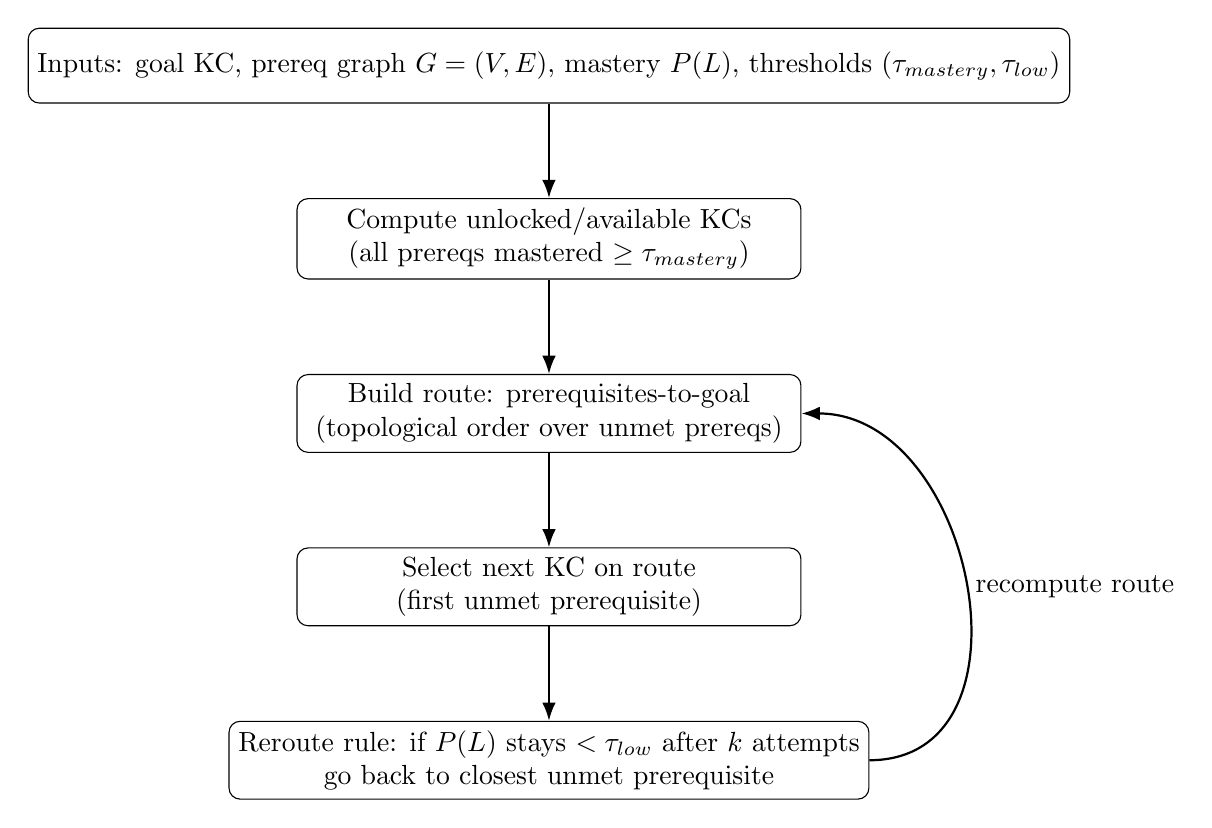
\begin{tikzpicture}[
  node distance=12mm,
  box/.style={draw, rounded corners, align=center, minimum width=6.4cm, minimum height=0.95cm},
  arrow/.style={-Latex, thick}
]
\node[box] (inputs) {Inputs: goal KC, prereq graph $G=(V,E)$, mastery $P(L)$, thresholds $(\tau_{mastery}, \tau_{low})$};
\node[box, below=of inputs] (unlock) {Compute unlocked/available KCs\\(all prereqs mastered $\ge \tau_{mastery}$)};
\node[box, below=of unlock] (buildroute) {Build route: prerequisites-to-goal\\(topological order over unmet prereqs)};
\node[box, below=of buildroute] (nextkc) {Select next KC on route\\(first unmet prerequisite)};
\node[box, below=of nextkc] (reroute) {Reroute rule: if $P(L)$ stays $< \tau_{low}$ after $k$ attempts\\go back to closest unmet prerequisite};

\draw[arrow] (inputs) -- (unlock);
\draw[arrow] (unlock) -- (buildroute);
\draw[arrow] (buildroute) -- (nextkc);
\draw[arrow] (nextkc) -- (reroute);
\draw[arrow] (reroute.east) .. controls +(2.2,0) and +(2.2,0) .. node[right]{recompute route} (buildroute.east);

\end{tikzpicture}
\caption{Routing and rerouting: prerequisite satisfaction and mastery-driven backtracking.}
\label{fig:routing-logic}
\end{figure}

\paragraph{Route construction (v1).}
Given a goal KC, the engine computes the set of unmet prerequisites (backward graph traversal), topologically
orders them, and recommends the first unmet prerequisite as the next KC. This yields a transparent, debuggable
route consistent with prerequisite-based sequencing \cite{brusilovsky2001}.

\paragraph{Rerouting rule (v1).}
If a learner repeatedly fails to improve mastery on the current KC (e.g., $P(L) < \tau_{low}$ after $k$ attempts),
the system selects the closest unmet prerequisite (or the nearest ancestor KC not mastered) and recomputes the route.

\FloatBarrier

% ----------------------------
% 3.6 UI Screens (Conceptual)
% ----------------------------
\subsection{Learner User Interface (Conceptual)}
The learner UI is designed to make adaptation understandable. Rather than recommending items in an opaque way,
the UI visualizes the prerequisite map, indicates which nodes are unlocked, and explains why a KC is selected next.
Figure~\ref{fig:ui-flow} summarizes the primary screens.

\begin{figure}[H]
\centering
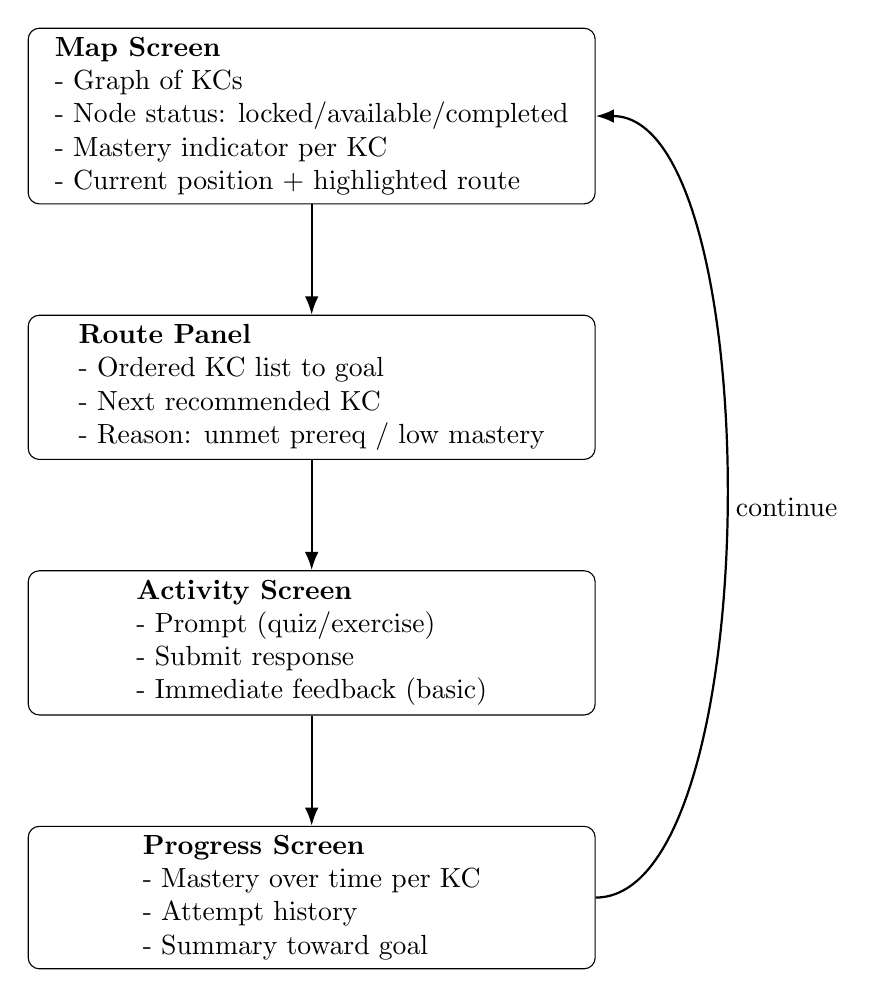
\begin{tikzpicture}[
  node distance=14mm,
  box/.style={draw, rounded corners, align=left, minimum width=7.2cm, minimum height=1.1cm},
  arrow/.style={-Latex, thick}
]
\node[box] (map) {\textbf{Map Screen}\\- Graph of KCs\\- Node status: locked/available/completed\\- Mastery indicator per KC\\- Current position + highlighted route};
\node[box, below=of map] (routepanel) {\textbf{Route Panel}\\- Ordered KC list to goal\\- Next recommended KC\\- Reason: unmet prereq / low mastery};
\node[box, below=of routepanel] (activity) {\textbf{Activity Screen}\\- Prompt (quiz/exercise)\\- Submit response\\- Immediate feedback (basic)};
\node[box, below=of activity] (progress) {\textbf{Progress Screen}\\- Mastery over time per KC\\- Attempt history\\- Summary toward goal};

\draw[arrow] (map) -- (routepanel);
\draw[arrow] (routepanel) -- (activity);
\draw[arrow] (activity) -- (progress);
\draw[arrow] (progress.east) .. controls +(2.2,0) and +(2.2,0) .. node[right]{continue} (map.east);
\end{tikzpicture}
\caption{Conceptual UI flow for a learner: map $\rightarrow$ route $\rightarrow$ activity $\rightarrow$ progress.}
\label{fig:ui-flow}
\end{figure}

\paragraph{Instructor/Admin UI (v1).}
The admin UI supports creating KCs, defining prerequisite edges, and authoring KC-tagged items. This enables
rapid iteration on the domain model while keeping the prerequisite structure explicit and editable.

\FloatBarrier

% ----------------------------
% 3.7 Deployment / Infra (Minimal)
% ----------------------------
\subsection{Deployment and Infrastructure (Minimal)}
The system can be deployed using a standard web stack with a hosted frontend, an API service, and a managed
relational database. Figure~\ref{fig:infra} illustrates a minimal deployment appropriate for a term-scale prototype.

\begin{figure}[H]
\centering
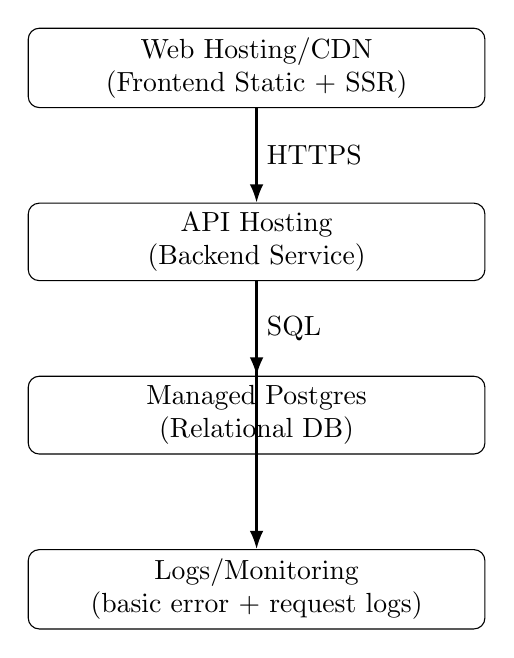
\begin{tikzpicture}[
  node distance=12mm,
  box/.style={draw, rounded corners, align=center, minimum width=5.8cm, minimum height=0.95cm},
  arrow/.style={-Latex, thick}
]
\node[box] (cdn) {Web Hosting/CDN\\(Frontend Static + SSR)};
\node[box, below=of cdn] (api) {API Hosting\\(Backend Service)};
\node[box, below=of api] (db) {Managed Postgres\\(Relational DB)};
\node[box, below=of db] (logs) {Logs/Monitoring\\(basic error + request logs)};

\draw[arrow] (cdn) -- node[right]{HTTPS} (api);
\draw[arrow] (api) -- node[right]{SQL} (db);
\draw[arrow] (api) -- (logs);
\end{tikzpicture}
\caption{Minimal deployment setup suitable for a term-scale prototype.}
\label{fig:infra}
\end{figure}

\paragraph{Logging.}
All learner interactions are persisted as append-only attempt events to support debugging, reproducibility, and
evaluation. Basic request/error logs are collected at the API layer.

\FloatBarrier

\section{Evaluation Plan}

When I started thinking about evaluation, I wanted to be honest with myself about what I could actually measure within a single-term project without real learner populations. Rather than simulate an experiment I couldn't run, I focused on three concrete validation goals: (1) verifying that the BKT implementation behaves correctly, (2) confirming that the routing and decision logic matches the intended policy, and (3) demonstrating that the end-to-end system works as designed through structured manual walkthroughs.

\subsection{BKT Sanity Checks}

The first thing I validated was the BKT update function itself. I wrote unit tests that trace mastery trajectories under controlled conditions:

\begin{itemize}
    \item A learner who answers every question correctly should cross $\tau_{mastery} = 0.95$ within a reasonable number of attempts given the default parameters ($P(L_0) = 0.10$, $P(T) = 0.10$, $P(G) = 0.25$, $P(S) = 0.10$). In practice, this happens in roughly 8--12 correct answers, which felt reasonable.
    \item A learner who answers every question incorrectly should see mastery stay low and eventually trigger the reroute condition ($P(L) < \tau_{low} = 0.40$ after $k = 3$ attempts).
    \item Mixed sequences (correct then incorrect) should produce intermediate trajectories that don't swing wildly, which they did.
\end{itemize}

These checks gave me confidence that the Bayesian update and learning transition were implemented correctly per the Corbett \& Anderson formulation \cite{corbett1995}. The parameters were taken directly from literature defaults rather than fit to data, which is a known limitation, but for a prototype without learner data, this is a reasonable starting point \cite{vandesande2013}.

\subsection{Routing and Decision Policy Validation}

The routing engine was validated through integration tests covering the following cases:

\begin{itemize}
    \item \textbf{Clean path to goal:} Given a learner with no mastered KCs targeting Recursion, the engine should return the full topologically-ordered path (Variables $\to$ Boolean Expressions $\to$ Conditionals $\to$ Loops $\to$ Functions $\to$ Recursion). It does.
    \item \textbf{Partial mastery:} If Variables and Boolean Expressions are already mastered, the route should begin at Conditionals. It does.
    \item \textbf{Reroute trigger:} After $k = 3$ attempts on a KC with $P(L) < 0.40$, the system should fall back to the nearest unmet prerequisite and recompute. This was verified both in unit tests and manually in the UI.
    \item \textbf{Goal already mastered:} If the learner already exceeds $\tau_{mastery}$ on the goal KC, no route should be generated. This edge case was handled correctly.
\end{itemize}

Each attempt response from the API also includes a plain-language \texttt{decision} field explaining \textit{why} the system made the choice it did (e.g., "Your mastery of Conditionals is now 0.97, advancing to Loops"). I treated this as a lightweight explainability check: if the rationale read correctly and consistently, the underlying logic was likely sound.

\subsection{End-to-End Walkthrough}

I ran several manual walkthroughs of the full learner flow to verify the system behaves coherently in practice. The scenario I used most was:

\begin{enumerate}
    \item Enter as a new learner with no prior history.
    \item Select Recursion as the goal.
    \item Work through the generated route, deliberately answering some questions incorrectly to trigger remediation and reroute.
    \item Verify that the map updates in real time, the mastery bar moves correctly, and the next KC recommendation matches what the decision policy should output.
\end{enumerate}

The system behaved as expected across all walkthroughs. The interactive knowledge graph (built with React Flow) rendered node states correctly: locked, in progress, and mastered nodes were visually distinct, and the AI tutor responses were contextually appropriate without ever interfering with the routing logic.

\subsection{Limitations of This Evaluation}

I want to be clear about what this evaluation does and does not show. Because I didn't have real learners, I can only verify correctness of implementation, not effectiveness as a learning tool. The BKT parameters were not fit to data, so mastery trajectories reflect literature defaults rather than calibrated estimates for this specific KC set. Whether $\tau_{mastery} = 0.95$ is the right threshold for advancing a learner in practice is an empirical question I wasn't able to answer in this term.

The most meaningful next step for evaluation would be a small pilot study with actual students, tracking whether the adaptive routes improve mastery acquisition relative to a fixed sequential curriculum. This would provide the kind of evidence that would let me iterate on thresholds, parameters, and routing heuristics with real signal rather than intuition.

\FloatBarrier

% ============================
% SECTION 5: RISKS & TIMELINE
% ============================

\section{Risks and Timeline}

\subsection{Risks and How They Played Out}

At the start of the project I identified several risks that I thought were most likely to derail the work. Looking back, some of them materialized in roughly the way I expected, and a few turned out to be non-issues.

\paragraph{BKT identifiability and parameter sensitivity.}
This was the risk I was most concerned about going in. The literature is clear that BKT can produce similar mastery curves from very different parameter sets, and without real learner data to fit against, I had no way to know whether my chosen parameters were realistic \cite{vandesande2013}. In practice, I mitigated this by choosing conservative defaults from Corbett \& Anderson \cite{corbett1995} and manually checking that mastery trajectories "felt right" under a variety of simulated answer sequences. It worked well enough for a prototype, but I'm aware that this is the weakest part of the system from a scientific standpoint. Any future work would need real data and proper parameter fitting.

\paragraph{Graph routing correctness with multi-path prerequisites.}
The prerequisite graph has one branching case: both Loops and Arrays/Lists are prerequisites for Recursion via different paths (Conditionals $\to$ Loops $\to$ Functions $\to$ Recursion and Conditionals $\to$ Functions $\to$ Arrays/Lists $\to$ Recursion). I was worried that the backward BFS + topological sort approach would produce incorrect or ambiguous routes at the merge point. In the end, the implementation handled this cleanly; the topological ordering correctly serialized both branches, but it took a few iterations to get right.

\paragraph{Frontend complexity and state synchronization.}
I underestimated how much state management complexity would emerge on the frontend once routing decisions needed to update the map, the mastery bar, and the next-activity recommendation simultaneously. Using Zustand with localStorage persistence helped, but there were some tricky bugs where stale state from a previous session would interfere with a new route. I fixed these, but it cost more time than I had budgeted.

\paragraph{AI tutor integration interfering with routing.}
Early on I was worried that integrating an LLM tutor might complicate the routing logic or create confusing interactions where the tutor's advice contradicted the system's recommendation. I resolved this cleanly by treating the tutor as a completely separate service: it reads the current KC context but has no write access to mastery, routes, or attempts. The routing logic is entirely deterministic and unaffected by whatever the tutor says. This architectural decision turned out to be the right one.

\paragraph{Risks that did not materialize.}
Database schema migrations were surprisingly smooth; Alembic handled all incremental changes without requiring manual intervention. Docker Compose setup, which I anticipated would be fiddly, worked reliably across clean installs. And the React Flow graph library handled the prerequisite DAG rendering much more gracefully than I expected.

\subsection{Timeline}

The project ran from early January to early April 2026 over approximately 13 weeks.

\begin{itemize}
    \item \textbf{Weeks 1--2 (Jan 5--18):} Literature review. Read Corbett \& Anderson (BKT), VanLehn (outer/inner loop), Brusilovsky (adaptive hypermedia), and surveyed DKT. Drafted the background sections of this report.
    \item \textbf{Weeks 3--4 (Jan 19 -- Feb 1):} System design. Defined the KC set, prerequisite graph structure, data model, and API contracts. Wrote up the proposed system design section.
    \item \textbf{Weeks 5--6 (Feb 2--15):} Core backend. Implemented the FastAPI skeleton, SQLAlchemy models, Alembic migrations, and the BKT service. Wrote unit tests for the update function.
    \item \textbf{Weeks 7--8 (Feb 16 -- Mar 1):} Routing engine and decision policy. Implemented backward BFS route generation, the advance/remediate/reroute policy, and the seed data (7 KCs, 7 edges, 28+ items).
    \item \textbf{Weeks 9--10 (Mar 2--15):} Frontend. Built the Next.js app with React Flow knowledge graph, Zustand store, and the core learner flow (landing $\to$ goal $\to$ map $\to$ practice $\to$ progress).
    \item \textbf{Weeks 11--12 (Mar 16--29):} Integration, AI tutor, admin UI, Docker Compose setup. Wired frontend to backend, added the optional LLM tutor panel, built the admin interface for managing KCs and items.
    \item \textbf{Week 13 (Mar 30 -- Apr 2):} Testing, evaluation walkthroughs, documentation, and report completion.
\end{itemize}

\FloatBarrier

% ============================
% CONCLUSION
% ============================

\section{Conclusion}

When I started this project I had a fairly abstract idea: build something like "Google Maps for learning", a system that knows where a learner is, knows where they want to go, and generates a route that adjusts as they move through the material. Thirteen weeks later, that idea is a working system.

The MVP implements the full adaptive loop as designed. A learner picks a goal KC, the system builds a personalized prerequisite-respecting route using backward BFS and topological sort, quiz items are served one at a time, and mastery is updated after every attempt using Bayesian Knowledge Tracing. The decision policy (advance when $P(L) \ge 0.95$, reroute when $P(L) < 0.40$ after three attempts) runs cleanly and produces routing decisions that are both sensible and explained to the learner in plain language. The interactive knowledge graph updates in real time, and the optional AI tutor (Claude by default) provides contextual explanation without ever touching the routing logic.

What I'm most satisfied with is that the system is genuinely interpretable. Every decision the system makes, whether to advance, remediate, or reroute, comes with a plain-language rationale that a learner can read and actually understand. This was a deliberate design priority from the beginning, and it held up through implementation. I didn't have to sacrifice transparency to make the adaptation work.

That said, I want to be honest about the limitations. The BKT parameters are literature defaults, not fitted values. Without real learner data, I have no way to know whether $\tau_{mastery} = 0.95$ is the right bar, or whether $P(T) = 0.10$ reflects how quickly students actually learn the KCs in the seed data. The expert-defined prerequisite graph is reasonable, but it's still one person's model of how CS concepts depend on each other, and a data-driven edge validation would strengthen it considerably. And the evaluation, while rigorous in terms of correctness testing, cannot answer the question that matters most: does this system actually help students learn better than a fixed curriculum would?

These are exactly the right questions to ask next. A small pilot study with real introductory CS students, tracking mastery trajectories, comparing adaptive routes against sequential ones, and gathering qualitative feedback on explainability, would provide the signal needed to move from a working prototype to a validated system. The infrastructure is built and ready for that kind of study.

Looking at the research literature I surveyed at the start, I think the design choices held up well. BKT turned out to be exactly the right model for a first implementation: transparent, implementable, and expressive enough to drive meaningful routing decisions without requiring data I didn't have. VanLehn's outer-loop framing was the right lens for thinking about the system's core responsibility \cite{vanlehn2006}. And Brusilovsky's observation that explicit prerequisite graphs enable both rerouting and explainability \cite{brusilovsky2001} proved true in practice; the graph structure is the thing that makes the system's recommendations legible to learners, not just technically correct.

The project met the goals I set out with. The adaptive learning system I described in January exists as a functional, tested, dockerized application in April. I learned a lot building it, from knowledge tracing and graph-based routing to how hard it is to synchronize frontend state with real-time backend decisions, and I think it's a solid foundation for future work in adaptive CS education.

% ============================
% REFERENCES
% ============================

\newpage
\begin{thebibliography}{99}

\bibitem{brusilovsky2001}
P.~Brusilovsky,
\textit{Adaptive Hypermedia},
User Modeling and User-Adapted Interaction, vol.~11, no.~1--2, pp.~87--110, 2001.
Available: \url{https://link.springer.com/article/10.1023/A:1011143116306}.

\bibitem{woolf2009}
B.~P.~Woolf,
\textit{Building Intelligent Interactive Tutors: Student-Centered Strategies for Revolutionizing E-Learning},
Morgan Kaufmann, San Francisco, CA, 2009.

\bibitem{vanlehn2006}
K.~VanLehn,
\textit{The Behavior of Tutoring Systems},
International Journal of Artificial Intelligence in Education, vol.~16, no.~3, pp.~227--265, 2006.
Available: \url{https://www.cs.colorado.edu/~mozer/Teaching/syllabi/6872/readings/VanLehn06.pdf}.

\bibitem{corbett1995}
A.~T.~Corbett and J.~R.~Anderson,
\textit{Knowledge Tracing: Modeling the Acquisition of Procedural Knowledge},
User Modeling and User-Adapted Interaction, vol.~4, no.~4, pp.~253--278, 1995.
Available: \url{https://link.springer.com/article/10.1007/BF01099821}.

\bibitem{piech2015dkt}
C.~Piech, J.~Bassen, J.~Huang, S.~Ganguli, M.~Sahami, L.~Guibas, and J.~Sohl-Dickstein,
\textit{Deep Knowledge Tracing},
Advances in Neural Information Processing Systems (NeurIPS), vol.~28, 2015.
Available: \url{https://stanford.edu/~cpiech/bio/papers/deepKnowledgeTracing.pdf}.

\bibitem{feng2014assistments}
M.~Feng, N.~Heffernan, and K.~Koedinger,
\textit{Addressing the Assessment Challenge with an Online System that Tutors as it Assesses},
Proceedings of the 7th International Conference on Educational Data Mining (EDM), 2014.
Available: \url{https://educationaldatamining.org/EDM2014/uploads/procs2014/FengHeffernanKoedinger.pdf}.

\bibitem{song1997}
J.~S.~Song, A.~M.~K.~Choi, and J.~Lee,
\textit{An Intelligent Tutoring System for Introductory C Language Programming},
Computers \& Education, vol.~28, no.~2, pp.~93--108, 1997.
Available: \url{https://www.sciencedirect.com/science/article/pii/S0360131597000031}.

\bibitem{vandesande2013}
B.~van~de~Sande,
\textit{Properties of the Bayesian Knowledge Tracing Model},
Journal of Educational Data Mining, vol.~5, no.~2, pp.~1--10, 2013.
Available: \url{https://jedm.educationaldatamining.org/index.php/JEDM/article/view/35}.

\bibitem{yudelson2013ibkt}
M.~V.~Yudelson, K.~R.~Koedinger, and G.~J.~Gordon,
\textit{Individualized Bayesian Knowledge Tracing Models},
Proceedings of the 16th International Conference on Artificial Intelligence in Education (AIED), pp.~171--180, 2013.
Available: \url{https://www.cs.cmu.edu/~ggordon/yudelson-koedinger-gordon-individualized-bayesian-knowledge-tracing.pdf}.

\bibitem{robins2003}
A.~Robins, J.~Rountree, and N.~Rountree,
\textit{Learning and Teaching Programming: A Review and Discussion},
Computer Science Education, vol.~13, no.~2, pp.~137--172, 2003.
Available: \url{https://www.tandfonline.com/doi/abs/10.1076/csed.13.2.137.14200}.

\bibitem{koedinger2012}
K.~R.~Koedinger, A.~T.~Corbett, and C.~Perfetti,
\textit{The Knowledge-Learning-Instruction Framework: Bridging the Science--Practice Chasm to Enhance Robust Student Learning},
Cognitive Science, vol.~36, no.~5, pp.~757--798, 2012.
Available: \url{https://onlinelibrary.wiley.com/doi/10.1111/j.1551-6709.2012.01245.x}.

\end{thebibliography}

\end{document}
